\documentclass{article}
\usepackage[utf8]{inputenc}
\usepackage[margin=1in]{geometry}
\usepackage{parskip}
\usepackage{alltt}
\usepackage{amsmath}
\usepackage{fixltx2e}
\usepackage{hyperref}
\usepackage{graphicx}

\begin{document}
\begin{flushright}
Samson Shi.354

\today

CSE 3461 Homework 1
\end{flushright}

\begin{enumerate}

\item[1]\textbf{(8 points)} Suppose users share a 3 Mbps link. Each user requires 150 kbps when transmitting, but each user transmits only 10\% of the time

\begin{enumerate}
\item \textbf{(2 points)} When circuit switching is used, how many users can be supported? 

20 Users can be supported because each user requires only 1/20th of the bandwith.

\item \textbf{(2 points)} Assume packet switching is used for the rest of this problem. Find the probability that a given user is transmitting.

The probability that a given user is transmitting is $P = 10\%$ since each user can only transmit 10\% of the time. 

\item \textbf{(2 points)} Suppose there are 120 users. Find the probability that exactly n users are transmitting simultaneously at any given time. (Hint: Use the binomial distribution.)

$P=\binom{120}{n} * 0.1^n * (0.9)^{120-n}$

\item \textbf{(2 points)} Find the probability that there are 21 or more users transmitting simultaneously.

$P = \sum_{\substack{n=0}}^{21} \binom{120}{n}0.1^n * 0.9^{120-n}$

\end{enumerate}

\item[2]\textbf{(8 points)} A client is fetching a base HTML file with $k$ referenced objects $(k > 0)$ from an Internet server. Let the RTT be $r$. Assume that the transmission/reception time for each file and referenced objects, if any, is $d$. Further, the only transmission/reception bottleneck in the network is the access link through which the client is connected to the Internet. In terms of $r, k,$ and $d$, compute the following delay for the following scenarios

\begin{enumerate}
\item \textbf{(2 points)} Non-persistent HTTP with parallel TCP connections (there is no limit on the number of parallel connections).

Assuming there isn't a limit on the number of parallel connections, the client would need $2*RTT$ time for the non-persistent HTTP connection and then add on the amount of time to retrieve just one object. (If there are $n$ objects and there is no limit on the number of parallel objects, the client could have $n$  parallel TCP connections, allowing it to download $n$ objects in the same time as downloading just one). Additionally, there is a cost of $d$ on the first HTML file. 

$Total Time = 2*r + 2*d$

\item \textbf{(2 points)} Non-persistent HTTP with no parallel TCP connections.

Without a parallel connection, the client would only have to make a $2*RTT$ trip for each object to download on a non-persistent connection as well as the intial setup cost.

$Total Time = 2*r*k*d + 2*r + d$

\item \textbf{(2 points)} Persistent HTTP with pipelining.

On a persitent HTTP connection, it just takes one RTT to set up a TCP connection. Then, it takes one more RTT to request the $k$ number of objects. Finally, the additional $d$ time for each object should be taken into consideration  as well as one RTT for the HTML file (which adds another $d$ time). 

$TotalTime = 3*r + k*d$

\item \textbf{(2 points)} Persistent HTTP without pipelining.

Without pipelining and with persistent HTTP, it would take one RTT to set up a TCP connection and then one RTT for each additioanl request and reply per object as well as one RTT for the HTML file (which adds another $d$ time).

$TotalTime = 2*r + (k*r*d) + d$

\end{enumerate}

\item[3]\textbf{(4 points)}Compare and contrast wired and wireless networks. You can find information in the textbook and online. Please cite all references you found.

The main difference between wired and wireless networks is that wireless networks require the usage of an access point from which to send and receive packets. The access point is then connected to the enterprise's network which is in turn connected to the wired Internet. A wired network, on the otherhand, uses copper wire ethernet cables to connect to an ethernet switch and is then connected to the wired Internet (Textbook, 17). While most people think of Wi-Fi when talking about wireless networks, cellular networks operate in a similar fashion, with available range being in the magnitude of kilometers, rather than 10s of meters.

Furthermore, in its current form, wireless networks are slower than wired networks as well and are more prone to security failure. Additionally, network types differ between wired and wireless networks. A wired network can take the form of a Local Area Network, Metropolitan Area Network, or a Wide Area Network. Wireless networks on the other hand can be ad hoc networks, wireless LAN/MAN/WAN networks as well as Wireless Personal Area networks, or be classified by their access technology such as GSM, TDMA, and CDMA. Additioanlly, networks can be classified by their radio access technology: Wi-Fi, Bluetooth, Infrared, and Hyperlan2. 

Source: \url{http://www.technicaljournalsonline.com/ijeat/VOL\%20V/IJAET\%20VOL\%20V\%20ISSUE\%20II\%20APRIL\%20JUNE\%202014/Article\%2009\%20V\%20II\%202014.pdf}

\item[4]\textbf{(6 points)} Consider the figure below. Answer the following questions. Assume we know the bottleneck link along the path from the server to the client is the first link with rate $R\textsubscript{S}$ bit/s. Suppose we send a pair of packets back to back from the server to the client and there is no other traffic on the path. Assume each packet has size $L$ bits and both links have the same propagation delay $d\textsubscript{prop}$.

\begin{enumerate}
\item \textbf{(3 points)} What is the packet inter-arrival time at the destination? That is, how much time elapses from when the last bit of the first packet arrives until the last bit of the second packet arrives?
\item \textbf{(3 points)} Now assume that the second link is the bottleneck link (i.e., $R\textsubscript{c} < R\textsubscript{s}$. Is it possible that the second packet queues at the input queue of the second link? Explain. Now suppose that the server sends the second packet $T$ seconds after sending the first packet. How large must $T$ be to ensure no queueing before the second link? Explain.  
\end{enumerate}

\item[5]\textbf{(8 points)} Read the \texttt{man} pages for \texttt{nslookup(1)} and \texttt{whois(1)}. If you are not very familiar with UNIX man pages, start with \texttt{man man}. For all parts below, describe the commands you use to obtain your answers.

\begin{enumerate}
\item \textbf{(2 points)} Use \texttt{nslookup} and send DNS queries to \texttt{www.cse.ohio-state.edu}. Search for Type A, NS, and MX records and summarize your findings.

To query, I ran the commands \texttt{nslookup -type=NS www.cse.ohio-state.edu}, \texttt{nslookup -type=MX www.cse.ohio-state.edu}, and \texttt{nslookup -type=A www.cse.ohio-state.edu}. For both NS and MX, the query returned information about mail servers where as the type A just returned the Server, the address, and name.

\item \textbf{(2 points)} Use \texttt{nslookup} to find a Web server that has multiple IP addresses. Does the server \texttt{www.osu.edu} have multiple IP addresses?

The server \texttt{www.osu.edu} does have multiple IP addresses.

\item \textbf{(2 points)} What are the names and IP addresses of the authoritative name servers for the following machines: \texttt{www.csail.mit.edu} and \texttt{cs.illinois.edu}?

\texttt{Name: www.csail.mit.edu}

\texttt{Address: 128.30.2.155}

\texttt{Name: cs.illinois.edu}

\texttt{Address: 130.126.112.119}

\item \textbf{(2 points)} What are the names and IP addresses of the machines on which email servers for the following recipients is running: \texttt{champion@cse.ohio-state.edu} and \texttt{person@cs.ucla.edu}? (If there are several mail server machines, provide information on only one).

\texttt{Name: cse.ohio-state.}

\texttt{Address: 164.107.112.224}


\texttt{Name: cs.ucla.edu}

\texttt{Address: 164.67.100.181}


\end{enumerate}

\item[6]\textbf{(6 points)} This question asks you to perform \texttt{traceroute} to various hosts. For all parts below, describe the commands you use to obtain your answers.

\begin{enumerate}
\item \textbf{(2 points)} Perform \texttt{traceroute} to two hosts, each in a different city in China. Submit a printout of the two \texttt{traceroute} operation from the site. How many links are the same in the two \texttt{traceroutes}? Is the transpacific link the same?

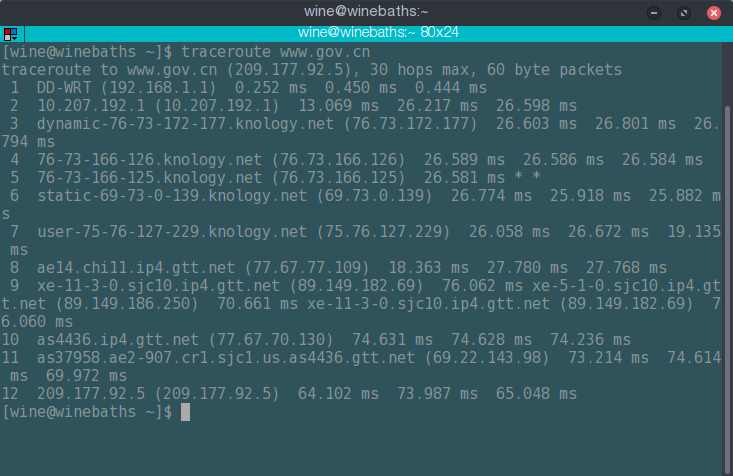
\includegraphics[scale=0.5]{cn1.png}

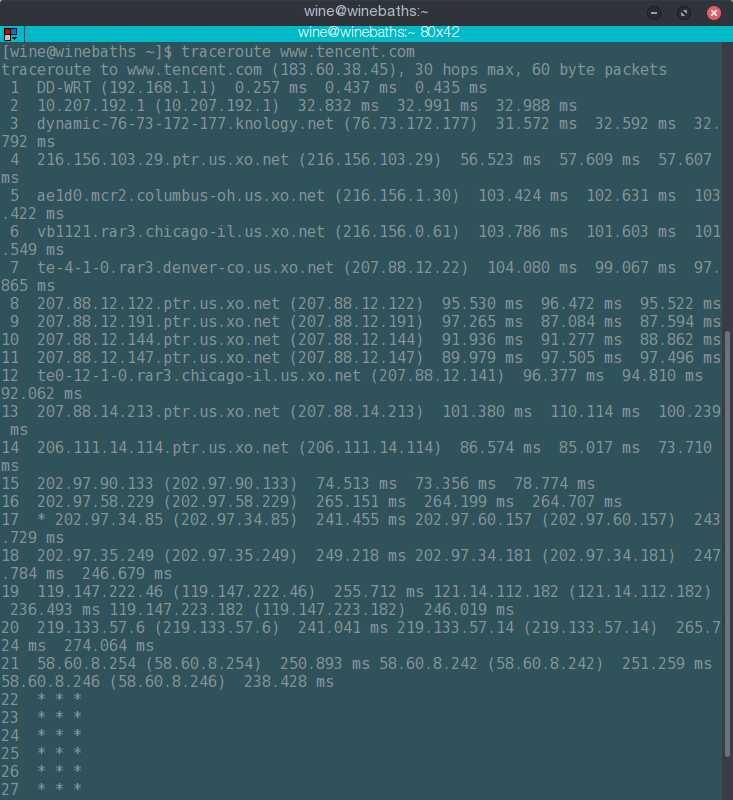
\includegraphics[scale=0.5]{cn2.png}

The only two links that are the same are the initial two. The transpacific link is not the same.

To get the traceroute, I ran the following commands;

\texttt{traceroute www.gov.cn}

\texttt{traceroute www.tencent.com}

\item \textbf{(2 points)} Repeat (a) but choose one city in china and another city in India.

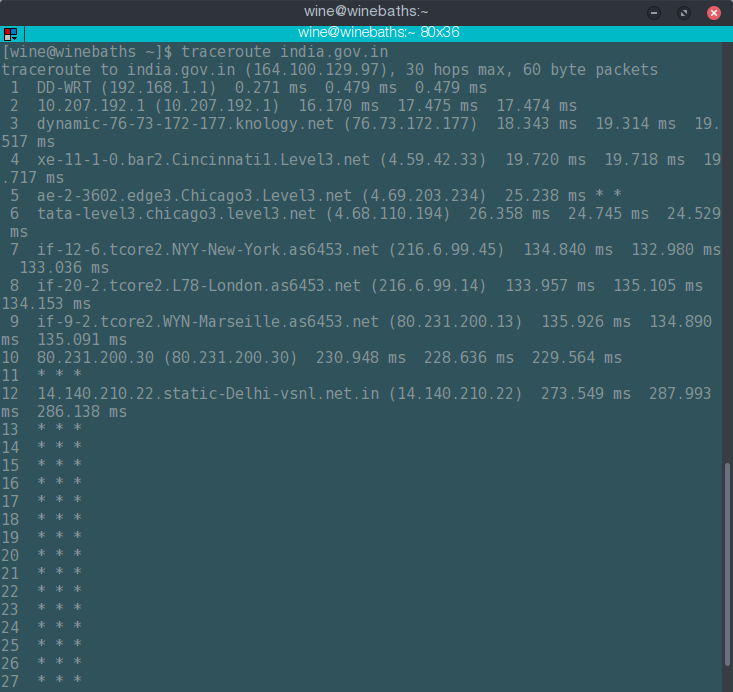
\includegraphics[scale=0.5]{in1.png}

\texttt{traceroute india.gov.in}

This traceroute shared another link with the \url{gov.cn} website, but none of them after that.

\item \textbf{(2 points)} Perform two \texttt{traceroutes} to two hosts, each in a different city in Europe. How many links are common to the two \texttt{traceroutes}? Do the \texttt{traceroutes} diverge before reaching Europe?

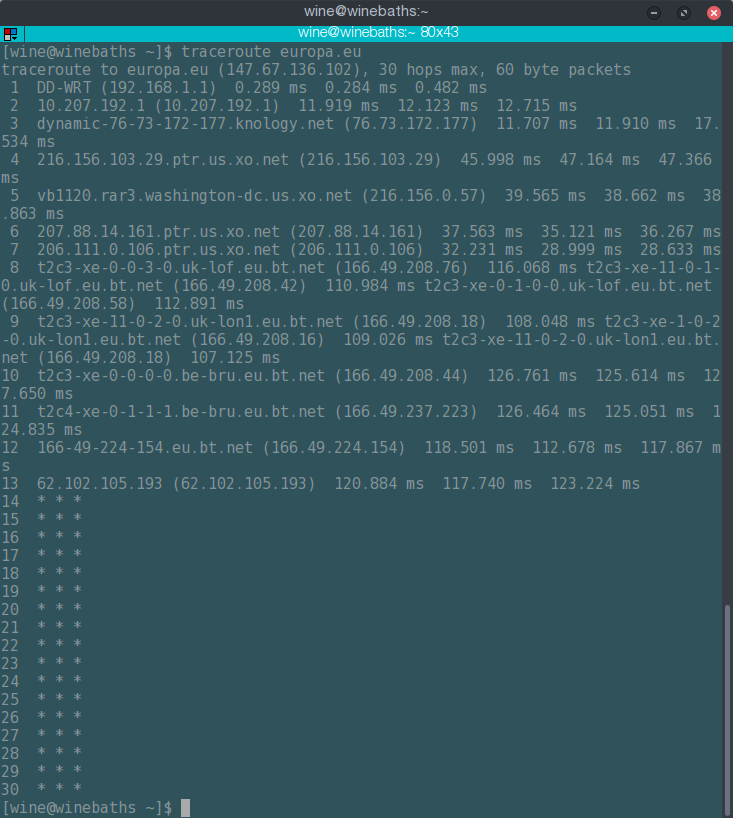
\includegraphics[scale=0.5]{eu1.png}

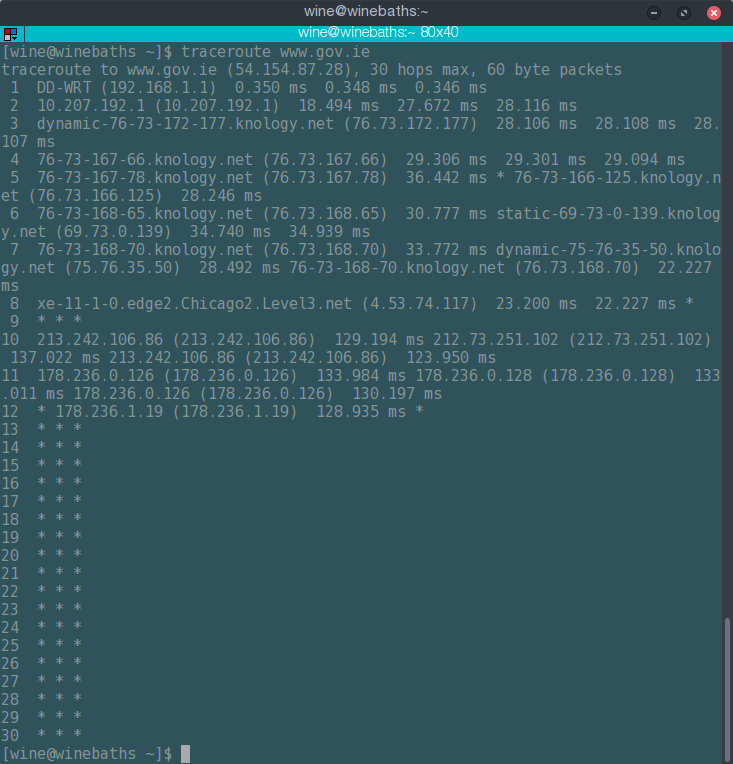
\includegraphics[scale=0.5]{ie1.png}

To get the traceroute, I ran the following commands;

\texttt{traceroute www.gov.ie}

\texttt{traceroute www.europa.eu}

The traceroutes diverge before getting to europe. The only two links that are common in the traceroute are the first two.
\end{enumerate}
\end{enumerate}

\end{document}